\documentclass[twoside]{article}
\setlength{\oddsidemargin}{0 in}
\setlength{\evensidemargin}{0 in}
\setlength{\topmargin}{-0.6 in}
\setlength{\textwidth}{6.5 in}
\setlength{\textheight}{8.5 in}
\setlength{\headsep}{0.75 in}
\setlength{\parindent}{0 in}
\setlength{\parskip}{0.1 in}

\usepackage{url}
\usepackage{titlesec}
\setcounter{secnumdepth}{3}
\usepackage{palatino}
\usepackage{marginnote}
\usepackage{multirow}
\usepackage{easybmat,bigdelim,arydshln}
\usepackage[authoryear,round]{natbib}
\usepackage{amssymb,amsmath,amsthm,amsfonts}
\usepackage{mathtools}
%\usepackage{nicematrix}
\usepackage{arydshln}
\usepackage{caption}
\usepackage{hyperref}
\usepackage{tcolorbox}
\tcbuselibrary{skins, breakable, theorems}
\usepackage{newpxtext,newpxmath}
\usepackage{longtable}
\usepackage{enumitem}
\makeatletter

\let\bar\overline

\setlist[itemize]{topsep=0pt,leftmargin=10pt,itemsep=-0.2em}
\usepackage{xcolor}
\usepackage{tikz}
\usepackage{pgfplots}
\pgfplotsset{compat = newest}
\usetikzlibrary{patterns,decorations.pathreplacing,decorations.markings,fit,shapes.geometric,angles,quotes,arrows}
\usepgfplotslibrary{fillbetween}

\usepackage{ifthen}
\usepackage{tikz-3dplot}

\pgfdeclarelayer{ft}
\pgfdeclarelayer{bg}
\pgfsetlayers{bg,main,ft}

\hypersetup{
    colorlinks,
    citecolor=red,
    filecolor=black,
    linkcolor=violet,
    urlcolor=blue
}

\definecolor{myblue}{cmyk}{1,.72,0,.38}
\definecolor{mypurple}{cmyk}{.57,1,0,.58}
\definecolor{myred}{cmyk}{0,.88,.88,.58}
\definecolor{mygreen}{cmyk}{1,0,.69,.66}
\definecolor{myorange}{cmyk}{0,.58,100,.20}
\definecolor{glaucous}{rgb}{0.38, 0.51, 0.71}

\makeatletter
\renewcommand{\thefigure}{\thesection.\arabic{figure}}
\newtheoremstyle{indented}
  {3pt}% space before
  {3pt}% space after
  {\addtolength{\@totalleftmargin}{3.5em}
   \addtolength{\linewidth}{-3.5em}
   \parshape 1 3.5em \linewidth}% body font
  {}% indent
  {\bfseries}% header font
  {.}% punctuation
  {.5em}% after theorem header
  {}% header specification (empty for default)
\makeatother

\newcommand{\ind}{\perp\!\!\!\perp}

\theoremstyle{definition}
\newtheorem{defin}{Definition}[section] % Creates a new counter, number within section
\newtheorem{prt}[defin]{Remark} 
\newtheorem{prts}[defin]{Remarks} % Again share defin's counter
\newtheorem{exmp}[defin]{Example} % etc.
\newtheorem{exmps}[defin]{Examples}
\newtheorem*{note}{Note}
\tcbuselibrary{theorems}

% use counter*=defin to make each tcbtheorem share defin's counter

\newtcbtheorem[use counter*=defin, number within=section]{definition}{Definition}{enhanced, breakable,
    colback = white, colframe = red!55!black, colbacktitle = red!55!black, attach boxed title to top left = {yshift = -2.5mm, xshift = 3mm}, boxed title style = {sharp corners},fonttitle=\bfseries}{def}

\newtcbtheorem[use counter*=defin, number within=section]{theorem}{Theorem}{enhanced, breakable,
    colback = white, colframe = blue!45!black, colbacktitle = blue!45!black, attach boxed title to top left = {yshift = -2.5mm, xshift = 3mm}, boxed title style = {sharp corners},fonttitle=\bfseries}{thm}
    
\newtcbtheorem[use counter*=defin, number within=section]{proposition}{Proposition}{enhanced, breakable,
    colback = white, colframe = teal, colbacktitle = teal, attach boxed title to top left = {yshift = -2.5mm, xshift = 3mm}, boxed title style = {sharp corners},fonttitle=\bfseries}{prop}

\newtcbtheorem[use counter*=defin, number within=section]{lemma}{Lemma}{enhanced, breakable,
    colback = white, colframe = orange!80!black, colbacktitle = orange!80!black, attach boxed title to top left = {yshift = -2.5mm, xshift = 3mm}, boxed title style = {sharp corners},fonttitle=\bfseries}{lemma}

\newtcbtheorem[use counter*=defin, number within=section]{example}{Example}{enhanced, breakable,
    colback = white, colframe = yellow!60!black, colbacktitle = yellow!60!black, attach boxed title to top left = {yshift = -2.5mm, xshift = 3mm}, boxed title style = {sharp corners},fonttitle=\bfseries}{exmp}

\newtcbtheorem[use counter*=defin, number within=section]{assumption}{Assumption}{enhanced, breakable,
    colback = white, colframe = violet!60!white, colbacktitle = violet!60!white, attach boxed title to top left = {yshift = -2.5mm, xshift = 3mm}, boxed title style = {sharp corners},fonttitle=\bfseries}{assump}

\newtcbtheorem[use counter*=defin, number within=section]{algorithm}{Algorithm}{enhanced, breakable,
    colback = white, colframe = green!55!black, colbacktitle = green!55!black, attach boxed title to top left = {yshift = -2.5mm, xshift = 3mm}, boxed title style = {sharp corners},fonttitle=\bfseries}{algm}
%\newtcolorbox{example}[1]{enhanced, breakable, colback = white, colframe = orange!85!black, colbacktitle = orange!85!black, attach boxed title to top left = {yshift = -2.5mm, xshift = 3mm}, boxed title style = {sharp corners},fonttitle=\bfseries, title={Example: #1}}

\newtcbox{\myhl}[1][white]
  {on line, arc = 0pt, outer arc = 0pt,
    colback = #1!20!white, colframe = #1!50!black,
    boxsep = 0pt, left = 1pt, right = 1pt, top = 1pt, bottom = 1pt, boxrule = 0pt, bottomrule =0pt, toprule =0pt}
    
\newtcbox{\myhlrule}[1][white]
  {on line, arc = 0pt, outer arc = 0pt,
    colback = #1!20!white, colframe = #1!50!black,
    boxsep = 0pt, left = 1pt, right = 1pt, top = 1pt, bottom = 1pt, boxrule = 0pt, bottomrule =0.5pt, toprule =0.5pt}
%
% The following commands set up the lecnum (lecture number)
% counter and make various numbering schemes work relative
% to the lecture number.
%
\newcounter{lecnum}
\renewcommand{\thepage}{\thelecnum-\arabic{page}}
\renewcommand{\thesection}{\thelecnum.\arabic{section}}
\renewcommand{\theequation}{\thelecnum.\arabic{equation}}
\renewcommand{\thefigure}{\thelecnum.\arabic{figure}}
\renewcommand{\thetable}{\thelecnum.\arabic{table}}

\newcommand{\sidenotes}[1]{\marginnote{\raggedright\scriptsize#1}}
%
% The following macro is used to generate the header.
%
\newcommand{\lecture}[6]{
   \pagestyle{myheadings}
   \thispagestyle{plain}
   \newpage
   \setcounter{lecnum}{#1}
   \setcounter{page}{1}
   \noindent
   \begin{center}
   \framebox{
      \vbox{\vspace{2mm}
    \hbox to 6.28in { {\bf Econometrics
	\hfill \today} }
       \vspace{4mm}
       \hbox to 6.28in { {\Large \hfill Topic #1: #2  \hfill} }
       \vspace{2mm}
       \hbox to 6.28in { {\it #3 \hfill by #4} }
      \vspace{2mm}}
   }
   \end{center}
   \markboth{Week #1: #2}{Week #1: #2}

   {\bf Key points}: {#5}

   {\bf Disclaimer}: {\it #6}
   \vspace*{4mm}
}
%

\tikzset{-stealth-/.style={decoration={
  markings,
  mark=at position #1 with {\arrow{stealth}}},postaction={decorate}}}

  \tikzset{tangent/.style={
    decoration={
        markings,% switch on markings
        mark=
            at position #1
            with
            {
                \coordinate (tangent point-\pgfkeysvalueof{/pgf/decoration/mark info/sequence number}) at (0pt,0pt);
                \coordinate (tangent unit vector-\pgfkeysvalueof{/pgf/decoration/mark info/sequence number}) at (1,0pt);
                \coordinate (tangent orthogonal unit vector-\pgfkeysvalueof{/pgf/decoration/mark info/sequence number}) at (0pt,1);
            }
    },
    postaction=decorate
},
use tangent/.style={
    shift=(tangent point-#1),
    x=(tangent unit vector-#1),
    y=(tangent orthogonal unit vector-#1)
},
use tangent/.default=1}

\tikzstyle{terminator} = [rectangle, draw, thick, text centered, rounded corners, minimum height=2em]
\tikzstyle{process} = [rectangle, draw, thick, text centered, minimum height=2em]
\tikzstyle{decision} = [diamond, draw, thick, text centered, minimum width=3cm, minimum height=0.5cm]
\tikzstyle{data}=[trapezium, draw, thick, text centered, trapezium left angle=60, trapezium right angle=120, minimum height=2em]
\tikzstyle{arrow} = [thick,->,>=stealth]

\begin{document}
\lecture{18}{Eigenvalue and Spike Models}{}{Sai Zhang}{.}{The note is built on Prof. \hyperlink{http://faculty.marshall.usc.edu/jinchi-lv/}{Jinchi Lv}'s lectures of the course at USC, DSO 607, High-Dimensional Statistics and Big Data Problems.}
%\footnotetext{These notes are partially based on those of Nigel Mansell.}

\section{Motivation}
Consider $n$ independent observations $\mathbf{X}_i\in \mathbb{R}^p$ drawn from a $\mathcal{N}(\mathbf{0},\boldsymbol{\Sigma})$, then the covariance can be decomposed into 2 parts, white noise and low rank
\begin{align*}
    \boldsymbol{\Sigma} = \mathrm{Cov}(\mathbf{X}_i) = \mathbf{I} + \sum^M_{k=1}\theta_k \nu_k\nu'_k =\boldsymbol{\Sigma}_0 + \boldsymbol{\Phi}
\end{align*}
where $M$ denotes the \myhl[myblue]{\textbf{number of spikes}} in the distribution of eigenvalues. The idea is: spikes deviate from a reference model along a \textbf{\underline{small fixed number}} of unknown directions. If $\boldsymbol{\Phi}=\mathbf{0}$, then none of the sample eigenvalues is separated from the bulk.

\paragraph*{Why a spike model is interesting?} A spike model can help determine the latent dimension of the data, some examples being
\begin{itemize}
    \item Principal component analysis (PCA): spikes are related to the directions of the most variations of the data, i.e., the principal components
    \item Clustering model: $M$ spikes is equivalent to $M+1$ clusters
    \item Economic significance: $M$ is related to the number of factor loadings
\end{itemize}

Then the question is threefold: 
\begin{itemize}
    \item[-] How to determine $M$
    \item[-] How to estimate $\nu_k$
    \item[-] How to test $\theta_k$
\end{itemize}

Under rank one alternative, we would like to test the hypothesis
$$
H_1: \boldsymbol{\Sigma} = \mathbf{I}_p+ \theta\boldsymbol{\nu}\boldsymbol{\nu}', \theta>0
$$
against the null
\begin{align*}
    H_0 &: \boldsymbol{\Sigma}= \mathbf{I}_p
\end{align*}
with the key assumptions:
\begin{itemize}
    \item[A1] Gaussian error
    \item[A2] large $p$: $p\leq n$ but allows $p/n \rightarrow \gamma \in (0,1)$ 
\end{itemize}
Under these assumptions, for the $n\times p$ data matrix $\mathbf{X} = \begin{pmatrix}
    \mathbf{X}'_1 &\cdots & \mathbf{X}'_n
\end{pmatrix}'$, $\mathbf{X}'\mathbf{X}$ has a $p-$dimensional \myhl[myblue]{\textbf{Wishart} distribution $W_p(n,\boldsymbol{\Sigma})$} with the degree of freedom $n$ and covariance matrix $\boldsymbol{\Sigma}$, which is a \textit{random matrix}.

If $\mathbf{Y} = \mathbf{M} + \mathbf{X}$, that is, the sum of the \textit{random matrix} $\mathbf{X}$ and a \textit{deterministic matrix} $\mathbf{M}$ (also $n\times p$), then $\mathbf{Y}'\mathbf{Y}$ has a $p-$dimensional Wishart distribution $W_p(n,\boldsymbol{\Sigma},\boldsymbol{\Psi})$ with $n$ degrees of freedom, covariance matrix $\boldsymbol{\Sigma}$ and non-centrality matrix $\boldsymbol{\Psi}=\boldsymbol{\Sigma}^{-1}\mathbf{M}'\mathbf{M}$.
\begin{definition}{Density of Wishart Distribution}{wishart_pdf}
    The PDF of Wishart distribution is defined as 
    \begin{align*}
        f(\mathbf{X}) = \frac{1}{2^{np/2}{\Gamma}_p\left(\frac{n}{2}\right)\left\vert \boldsymbol{\Sigma}\right\vert^{n/2} } \left\vert \mathbf{X} \right\vert^{(n-p-1)/2}\exp \left(-\frac{1}{2}\mathrm{tr}\left(\boldsymbol{\Sigma}^{-1}\mathbf{X}\right)\right)
    \end{align*}
    where $\mathbf{X}$ is a symmetric positive semidefinite and ${\Gamma}_p\left(\frac{n}{2}\right)$ is a multivariate gamma function such that 
    \begin{align*}
        {\Gamma}_p\left( \frac{n}{2} \right) = \pi^{\frac{p(p-1)}{4}} \prod^p_{j=1}{\Gamma}\left(\frac{n}{2}-\frac{j-1}{2}\right)
    \end{align*}
    Notice that the sample covariance matrix $\mathbf{S}=\frac{1}{n}\mathbf{X}'\mathbf{X}$ is just a scaled version of Wishart distribution
    $$
        n\mathbf{S} = \mathbf{X}'\mathbf{X} \sim W_p(n,\boldsymbol{\Sigma})
    $$
\end{definition}
For $\boldsymbol{\Sigma}=\mathbf{I}_p$, the empirical distribution fo eigenvalues converges to Marcenko-Pastur distribution
\begin{align*}
    f^{\mathrm{MP}}(x) = \frac{1}{2\pi\gamma x}\sqrt{(b_+-x)(x-b_-)}
\end{align*}
where $b_{\pm} = (1\pm \sqrt{\gamma})^2$. Then:
\begin{itemize}
    \item under $H_0: \boldsymbol{\Sigma}= \mathbf{I}_p$, we have 
    $$
    n^{2/3}\left( \frac{\lambda_1 -\mu(\gamma)}{\sigma (\gamma)} \right) \xrightarrow{d} \mathrm{TW}_1
    $$
    where $\mathrm{TW}_1$ is the Tracy-Widom distribution
    \item under $H_1: \boldsymbol{\Sigma} = \mathbf{I}_p+ \theta\boldsymbol{\nu}\boldsymbol{\nu}', \theta>0$, if $\theta$ is strong ($\theta\gg \sqrt{\gamma}$), then
    $$
    n^{1/2}\left( \frac{\lambda_1 - \rho(\theta,\gamma)}{\tau (\theta,\gamma)} \right) \xrightarrow{d}\mathcal{N}(0,1)
    $$
\end{itemize}
Here, the largest eigenvalue test is the best test. \textbf{But} when the signal is weak $(0 \leq \theta < \sqrt{\gamma})$, the largest eigenvalue under the alternative converges to the same distribution as null: 
\begin{align*}
    n^{2/3} \left( \frac{\lambda_1 - \rho(\theta,\gamma)}{\tau (\theta,\gamma)} \right) \xrightarrow{d} \mathrm{TW}_1
\end{align*}
which means that the largest eigenvalue test \textit{fails}. On top of this, \textbf{resampling} also fails when $p$ is large.
\begin{figure}[ht]
    \centering
    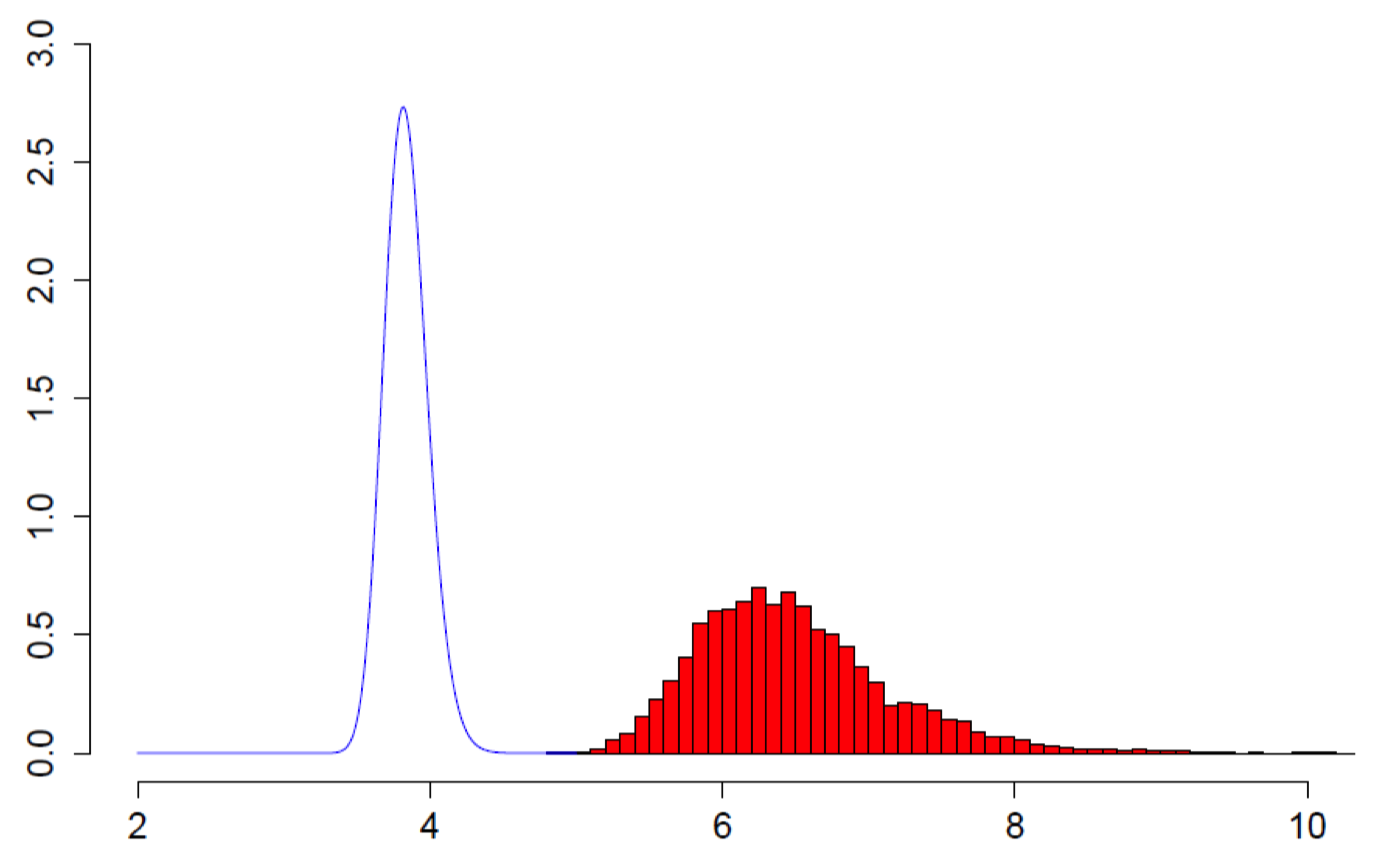
\includegraphics[width = 0.6 \textwidth]{figures/note18_resamplingfail.png}
    \caption{Failure of Resampling Test $(n=p=100)$}\label{fig:resampling_failure}
\end{figure}

Next, we develop another test to cope with these problems.

\section{Johnstone and Onatski (2020)}
Consider the basic equation of classical multivariate statistics:
\begin{align}\label{eq:multivariate_statistic}
    \det \left( \mathbf{H}-\mathbf{xE}\right) = 0
\end{align}
with $p\times p$ matrices
\begin{align*}
    n_1\mathbf{H} &= \sum^{n_1}_{k=1}\mathbf{x}_k\mathbf{x}_k' &\text{\textit{hypothesis} SS}\\
    n_1\mathbf{E} &= \sum^{n_1}_{k=1}\mathbf{z}_k\mathbf{z}_k' &\text{\textit{error} SS}
\end{align*}
The solution $\mathbf{x}$ is generalized eigenvalues $\left\{ \lambda_i \right\}^p_{i=1}$, which are the eigenvalue of \myhl[myblue]{F-ratio} $\mathbf{E}^{-1}\mathbf{H}$. \citet{johnstone2020testing} summarized 5 topics using $\mathbf{E}^{-1}\mathbf{H}$ relying on the five most common hypergeometric functions\footnote{Hypergeometric functions are:
\begin{itemize}
\item scalar inputs $$ _{\mathrm{p}}\mathcal{F}_{\mathrm{q}}(a,b;x) = \sum^{\infty}_{k=0} \frac{(a_1)_k\cdots (a_p)_k}{(b_1)_k\cdots (b_p)_k}\frac{x^k}{k!} $$ where $(a_j)_k$ are generalized Pochhammer symbols
\item single matrix inputs, where $\mathbf{S}$ is symmetric and usually diagonal $$ _{\mathrm{p}}\mathcal{F}_{\mathrm{q}}(a,b;\mathbf{S}) = \sum^{\infty}_{k=0} \sum_{\kappa} \frac{(a_1)_{\kappa}\cdots (a_p)_{\kappa}}{(b_1)_{\kappa}\cdots (b_p)_{\kappa}}\frac{C_{\kappa}(\mathbf{S})}{k!}  $$ where $C_k$ are the zonal polynomials. Easily, $ _{\mathrm{0}}\mathcal{F}_{\mathrm{0}}(\mathbf{S}) = e^{\mathrm{tr}(\mathbf{S})}$, $ _{\mathrm{1}}\mathcal{F}_{\mathrm{0}}(a,\mathbf{S}) = \left\vert \mathbf{I-S} \right\vert^{-a}$
\item two matrix inputs, where $\mathbf{S,T}$ are both symmetric $$ _{\mathrm{p}}\mathcal{F}_{\mathrm{q}}(a,b;\mathbf{S,T})  = \int_{O(p)} {}_{\mathrm{p}}\mathcal{F}_{\mathrm{q}} (a,b;\mathbf{SUTU'})\mathrm(d)\mathbf{U} $$
\end{itemize} } $_{\mathrm{p}}\mathcal{F}_{\mathrm{q}}$

\begin{table}[ht]
    \caption{5 Statistical Methods}\label{tab:5cases_James}
    \footnotesize
    \begin{center}
      \begin{tabular}{lccccc}
        
        \multicolumn{3}{c}{Statistical method} & $n_1\mathbf{H}$ & $n_2\mathbf{E}$ & Univariate Analog \\
        \hline
        $_{\mathrm{0}}\mathcal{F}_{\mathrm{0}}$ & PCA & Principal components analysis & $W_p(n_1,\boldsymbol{\Sigma+\Phi})$ & $n_2\boldsymbol{\Sigma}$ & $\chi^2$\\
        $_{\mathrm{1}}\mathcal{F}_{\mathrm{0}}$ & SigD & Signal detection & $W_p(n_1,\boldsymbol{\Sigma+\Phi})$ & $W_p(n_2,\boldsymbol{\Sigma})$ & non-central $\chi^2$ \\
        $_{\mathrm{0}}\mathcal{F}_{\mathrm{1}}$ & REG$_0$ & Multivariate regression, with known error & $W_p(n_1,\boldsymbol{\Sigma},n_1\boldsymbol{\Phi})$ & $n_2\boldsymbol{\Sigma}$ & $F$ \\
        $_{\mathrm{1}}\mathcal{F}_{\mathrm{1}}$ & REG & Multivariate regression, with unknown error & $W_p(n_1,\boldsymbol{\Sigma},n_1\boldsymbol{\Phi})$ & $W_p(n_2,\boldsymbol{\Sigma})$ & non-central $F$ \\
        $_{\mathrm{2}}\mathcal{F}_{\mathrm{1}}$ & CCA & Canonical correlation analysis & $W_p(n_1,\boldsymbol{\Sigma},\boldsymbol{\Phi}(\mathbf{Y}))$ & $W_p(n_2,\boldsymbol{\Sigma})$ & $\frac{r^2}{1-r^2}$\\ \hline
        \multicolumn{5}{l}{For $_{\mathrm{0}}\mathcal{F}_{\mathrm{0}}$ and $_{\mathrm{0}}\mathcal{F}_{\mathrm{1}}$, $\mathbf{E}$ is deterministic, $\boldsymbol{\Sigma}$ is known, $n_2$ disppears, otherwise $\mathbf{E}$ is independent of $\mathbf{H}$.}
      \end{tabular}
    \end{center}
\end{table}

\subsection{Definitions and global assumptions}
Let $\mathbf{Z}$ be an $n\times p$ data matrix with rows (observations) drawn \textbf{i.i.d.} from $\mathcal{N}_p(\mathbf{0},\boldsymbol{\Sigma})$, and a deterministic matrix $\mathbf{M}$ of $n\times p$, then for $\mathbf{Y} = \mathbf{M}+ \mathbf{Z}$, 
\begin{itemize}
    \item $\mathbf{H} = \mathbf{Y'Y}$ has a $p$ dimensional Wishart distribution $W_p(n,\boldsymbol{\Sigma,\Psi})$ with $n$ degrees of freedom, covariance matrix $\boldsymbol{\Sigma}$ and non-centrality matrix $\boldsymbol{\Psi}=\boldsymbol{\Sigma}^{-1}\mathbf{M'M}$
    \item the corresponding central Wishart distribution with $\mathbf{M}=\mathbf{0}$ is $W_p(n,\boldsymbol{\Sigma})$
\end{itemize}
\citet{johnstone2020testing} assume a relative low dimensionality $p\leq \min\left\{ n_1,n_2 \right\}$ where $n_1,n_2$ are the degrees of freedom as in Table \ref{tab:5cases_James}, where 
\begin{itemize}
    \item[-] $p\leq n_2$ ensures almost sure invertibility of matrix $\mathbf{E}$ in Equation \ref{eq:multivariate_statistic} 
    \item[-] $p\leq n_1$ is not essential, but reduces the number of various situations of consideration.
\end{itemize}

\subsection{5 classes of problems}
With these assumptions, they established a unified statistical problem \myhl[myblue]{\textbf{symmetric matrix denoising (SMD)}} that can be linked to the 5 classes of problems:

\paragraph*{PCA} $n_1$ i.i.d. observations drawn from $\mathcal{N}_p(\mathbf{0},\boldsymbol{\Omega})$ to test the hull hypothesis that the population covariance $\boldsymbol{\Omega} = \boldsymbol{\Sigma}$, with the alternative of interest being $$ \boldsymbol{\Omega} = \boldsymbol{\Sigma+\Phi},\ \text{ with }\boldsymbol{\Phi}=\theta \boldsymbol{\phi\phi'}  $$ where $\theta>0$, $\boldsymbol{\phi}$ are unknown, and $\boldsymbol{\phi}$ is normalized s.t. $\left\Vert \boldsymbol{\Sigma}^{-1/2}\boldsymbol{\phi} \right\Vert = 1$. W.L.O.G., assume $\boldsymbol{\Sigma}=\mathbf{I}_p$, then under the alternative, the first principal component explains a larger portion of the variation than the other principal components. Re-formulate the hypotheses in terms of the spectral \textit{spike} parameter $\theta$, we have
\begin{align}\label{eq:spectral_spike_hypotheses}
    H_0: \theta_0 &= 0 & H_1: \theta_0 = \theta>0
\end{align}
where $\theta_0$ is the true value of the \textit{spike}. A \myhl[myblue]{\textbf{maximal invariant statistic}} consists of the solutions $\lambda_1\geq \cdots\geq \lambda_p$ of Equation \ref{eq:multivariate_statistic} with
\begin{itemize}
    \item $n_1\mathbf{H}$ equal to the sample covariance matrix
    \item $\mathbf{E} = \boldsymbol{\Sigma}$
\end{itemize}

\paragraph*{SigD} Now consider testing the \textbf{equality} of covariance matrices $\boldsymbol{\Omega}$ and $\boldsymbol{\Sigma}$, corresponding to 2 independent $p-$dimensional mean-zero Gaussian samples of size \myhl[myblue]{$n_1$} and \myhl[myblue]{$n_2$}, with the alternative still  $$ \boldsymbol{\Omega} = \boldsymbol{\Sigma+\Phi},\ \text{ with }\boldsymbol{\Phi}=\theta \boldsymbol{\phi\phi'}  $$ and again, assume $\boldsymbol{\Sigma}=\mathbf{I}_p$ (but NOT necessarily known), here, instead of Equation \ref{eq:multivariate_statistic}, consider 
\begin{align}
    \det \left( \mathbf{H}-\boldsymbol{\lambda}\left(\mathbf{E}+\frac{n_1}{n_2}\mathbf{H}\right) \right) = 0
\end{align}
naturally, SigD reduces to PCA as $n_2\rightarrow\infty$ while $n_1$ and $p$ held constant.

\paragraph*{REG$_0$} Next, consider a linear regression with multivariate response $$ \mathbf{Y} = \mathbf{X}\boldsymbol{\beta} + \boldsymbol{\epsilon} $$ with known covariance matrix $\boldsymbol{\Sigma}$ of the i.i.d. Gaussian rows of the error matrix $\boldsymbol{\epsilon}$. Here, to test linear restrictions on the matrix of coefficients $\boldsymbol{\beta}$, we can split the matrix of transformed response variables $\mathbf{Y}$ into 3 parts $\mathbf{Y}_1,\mathbf{Y}_2,\mathbf{Y}_3$, where 
\begin{itemize}
    \item $\mathbf{Y}_1$ is $n_1\times p$ where $p$ is the number of response variables, $n_1$ is the number of linear restrictions (per each of the $p$ columns of matrix $\boldsymbol{\beta}$), under the null $H_0: \mathbb{E}\mathbf{Y}_1 = 0$, versus the alternative \begin{align}\label{eq:REG_alternative}
        \mathbb{E}\mathbf{Y}_1 = \sqrt{n_1\theta}\boldsymbol{\psi\phi'}
    \end{align}
    where $\theta>0$, $\left\Vert \boldsymbol{\Sigma}^{-1/2}\boldsymbol{\phi}\right\Vert = 1$ and $\lVert \boldsymbol{\psi}\rVert = 1$
    \item $\mathbf{Y}_2$ is $(q-n_1)\times p$, where $q$ is the number of regressors
    \item $\mathbf{Y}_3$ is $(T-q)\times p$, where $T$ is the number of observations
\end{itemize}
In this case, tests can be based on the solutions $\lambda_1,\cdots,\lambda_p$ to $$ \det \left( \mathbf{H}-\boldsymbol{\lambda }\mathbf{E} \right)=\mathbf{0} $$
where $\mathbf{H} = \mathbf{Y}'_1\mathbf{Y}_1/n_1$ and $\mathbf{E}=\boldsymbol{\Sigma}$. The solutions represent a multivaraite analog of the difference between the sum of squared residuals in the restircted and unrestricted regressions. Under the null, $n_1\mathbf{H}$ is distributed as $W_p(n_1,\boldsymbol{\Sigma})$. Here, 
\begin{align*}
    n_1\mathbf{H} & \sim W_p(n_1,\boldsymbol{\Sigma}) & \text{under }H_0\\
    n_1\mathbf{H} & \sim W_p(n_1,\boldsymbol{\Sigma},n_1\boldsymbol{\Phi}),\ \text{where }\boldsymbol{\Phi} = \theta \boldsymbol{\Sigma}^{-1}\boldsymbol{\phi\phi}' & \text{under }H_1
\end{align*}
Again, W.L.O.G, assume $\boldsymbol{\Sigma} = \mathbf{I}_p$. This \myhl[myblue]{\textbf{canonical form}} of REG$_0$ is essentially equivalent to the setting of \textbf{\underline{matrix denoising}}
$$
\mathbf{Y}_1 = \mathbf{M}+ \mathbf{Z}
$$

\paragraph*{REG} Again, consider the linear regression $$ \mathbf{Y} = \mathbf{X}\boldsymbol{\beta} + \boldsymbol{\epsilon} $$ but \textbf{NOT} knowing the covariance matrix $\boldsymbol{\Sigma}$ of rows of $\boldsymbol{\epsilon}$. Here, the solutions again solve $\det \left( \mathbf{H}-\boldsymbol{\lambda }\mathbf{E} \right)=\mathbf{0}$ with $$ \mathbf{H} = \mathbf{Y}'_1\mathbf{Y}_1/n_1,\ \mathbf{E}=\mathbf{Y}'_3\mathbf{Y}_3/n_2 $$
this represents a multivariate analog of the $F$ ratio: the difference between the sum of squared residuals in the restricted and unrestricted regressions to the sum of squared residuals in the restricted regression. Again, as $n_2 \rightarrow \infty$, REG reduces to REG$_0$. 

\paragraph*{CCA} Consider testing for independence between Gaussian vectors $x_t\in\mathbb{R}^p$ and $y_t\in \mathbb{R}^{n_1}$, given zero-mean observations with $t=1,\cdots,n_1+n_2$. Partition the population and sample covariance matrices of the observations $(x_t',y_t')'$ into 
\begin{align*}
    \begin{pmatrix}
        \boldsymbol{\Sigma}_{xx} & \boldsymbol{\Sigma}_{xy}\\
        \boldsymbol{\Sigma}_{yx} & \boldsymbol{\Sigma}_{yy}
    \end{pmatrix} & & \begin{pmatrix}
        \mathbf{S}_{xx} & \mathbf{S}_{xy}\\
        \mathbf{S}_{yx} & \mathbf{S}_{yy}
    \end{pmatrix}
\end{align*}
respsectively. Under $H_0:\boldsymbol{\Sigma}_{xy}=\mathbf{0}$, while the alternative is
\begin{align}
    \boldsymbol{\Sigma}_{xy} = \sqrt{\frac{n_1\theta}{n_1\theta + n_1 + n_2}}\boldsymbol{\phi\psi}'
\end{align}
where the nuisance parameters $\phi \in \mathbb{R}^p$ and $\psi \in \mathbb{R}^{n_1}$ are normalized s.t.
\begin{align*}
    \left\Vert \boldsymbol{\Sigma}_{xx}^{-1/2}\boldsymbol{\phi} \right\Vert = \left\Vert \boldsymbol{\Sigma}_{yy}^{-1/2}\boldsymbol{\psi} \right\Vert = 1
\end{align*}
And the test can be based on the squared sample canonical correlations $\lambda_1,\cdots,\lambda_p$ that solves $$ \det \left( \mathbf{H}-\boldsymbol{\lambda }\mathbf{E} \right)=\mathbf{0} $$
with
\begin{align*}
    \mathbf{H} &= \mathbf{S}_{xy}\mathbf{S}_{yy}^{-1}\mathbf{S}_{yx} & \mathbf{E}&\mathbf{S}_{xx}
\end{align*}

\subsection{SMD}
For a $\mathbf{X} = \boldsymbol{\Phi} + \mathbf{Z}/\sqrt{p}$ where $\mathbf{Z}$ is a noise matrix from the \myhl[myblue]{\textbf{Gaussian Orthogonal Ensemble} (GOE)}\footnote{$\mathbf{Z}$ is from the GOE that it is \textbf{symmetric} and \begin{align*} \mathbf{Z}_{ii} &\sim \mathcal{N}(0,2) & \mathbf{Z}_{ij}\sim\mathcal{N}(0,1) \text{ if }i>j \end{align*} }
We seek to make inference about a symmetric rank-one \textit{signal} matrix $\boldsymbol{\Phi} = \theta\boldsymbol{\phi\phi}'$. The null and the alternative is again as in \ref{eq:spectral_spike_hypotheses}. The nuisance vector $\boldsymbol{\phi}\in\mathbb{R}^p$ is normalized s.t. $\left\Vert \boldsymbol{\phi} \right\Vert =1$. 

The problem remains \myhl[myblue]{\textbf{invariant}} under the multiplication of $\mathbf{X}$ from the left by an orthogonal matrix, and from the right by its transpose.
A maximal invariant statistic consists of the solutions $\lambda_1,\cdots,\lambda_p$ to $\det \left( \mathbf{H}-\boldsymbol{\lambda }\mathbf{E} \right)=\mathbf{0} $ with $\mathbf{H}=\mathbf{X}$ and $\mathbf{E}=\mathbf{I}_p$.

SMD can be viewed as a degenerate version of the 5 classes of problems, as shown in Figure \ref{fig:smd_5classesofproblems}:
\begin{itemize}
    \item \myhl[myblue]{\textbf{SMD}}, \myhl[myblue]{\textbf{PCA}}, \myhl[myblue]{\textbf{REG$_0$}}: random $\mathbf{H}$ and deterministic $\mathbf{E}$
    \item \myhl[myblue]{\textbf{PCA}} and \myhl[myblue]{\textbf{SigD}} are \textit{parallel} to \myhl[myblue]{\textbf{REG$_0$}}
    \item \myhl[myblue]{\textbf{CCA}} has a different structure of $\mathbf{H}$ and $\mathbf{E}$
\end{itemize}

\begin{figure}[ht]
    \caption{SMD and 5 Classes of Statistical Problems}\label{fig:smd_5classesofproblems}
    \centering
      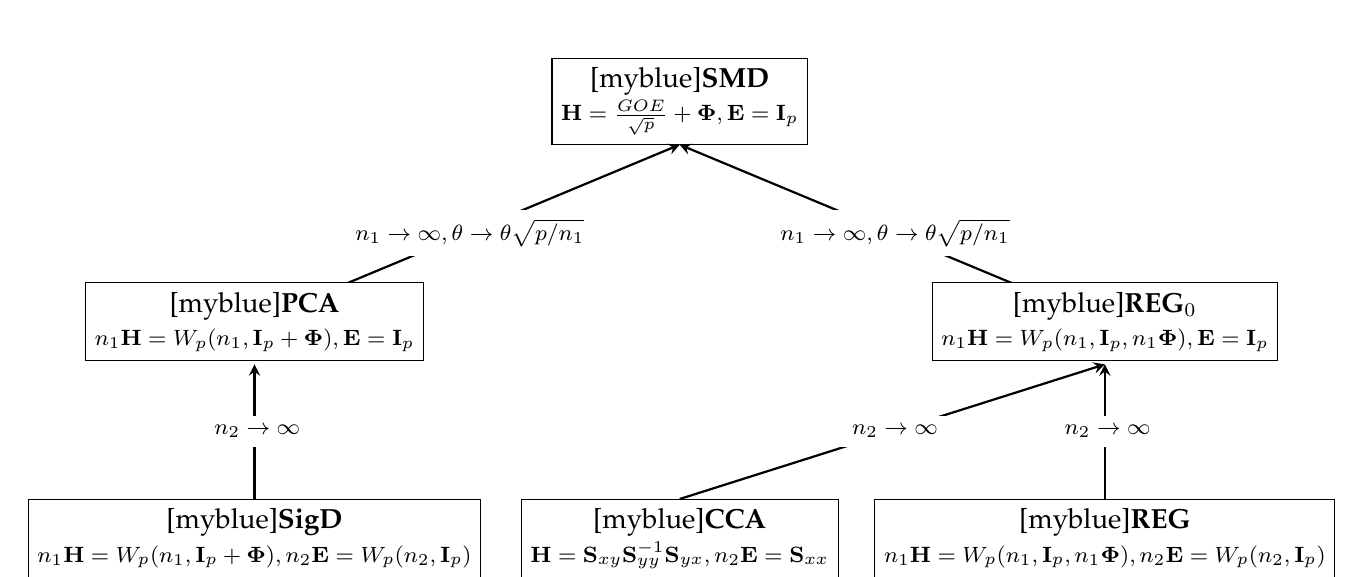
\begin{tikzpicture}[scale=0.9]
        \node[draw, above, align=center,fill=white] at (6,5) {\myhl[myblue]{\textbf{SMD}} \\ \footnotesize{$\mathbf{H}=\frac{GOE}{\sqrt{p}}+\boldsymbol{\Phi},\mathbf{E}=\mathbf{I}_p$}};
        
        \draw [-stealth,color=black,thick] (0,2.5) -- (6,5) node[midway, fill=white] {\footnotesize{ $n_1\rightarrow\infty,\theta\rightarrow\theta\sqrt{p/n_1}$ }};
        \node[draw, align=center,fill=white] at (0,2.5) {\myhl[myblue]{\textbf{PCA}} \\ \footnotesize{$n_1\mathbf{H}=W_p(n_1,\mathbf{I}_p+\boldsymbol{\Phi}),\mathbf{E}=\mathbf{I}_p$}};

        \draw [-stealth,color=black,thick] (12,2.5) -- (6,5) node[midway, fill=white] {\footnotesize{ $n_1\rightarrow\infty,\theta\rightarrow\theta\sqrt{p/n_1}$ }};
        \node[draw, align=center,fill=white] at (12,2.5) {\myhl[myblue]{\textbf{REG$_0$}} \\ \footnotesize{$n_1\mathbf{H}=W_p(n_1,\mathbf{I}_p,n_1\boldsymbol{\Phi}),\mathbf{E}=\mathbf{I}_p$}};

        \draw [-stealth,color=black,thick] (0,0) -- (0,1.9) node[midway, fill=white] {\footnotesize{ $n_2\rightarrow\infty$ }};
        \node[draw, below, align=center,fill=white] at (0,0) {\myhl[myblue]{\textbf{SigD}} \\ \footnotesize{$n_1\mathbf{H}=W_p(n_1,\mathbf{I}_p+\boldsymbol{\Phi}),n_2\mathbf{E}=W_p(n_2,\mathbf{I}_p)$}};

        \draw [-stealth,color=black,thick] (12,0) -- (12,1.9) node[midway, fill=white] {\footnotesize{ $n_2\rightarrow\infty$ }};
        \node[draw, below, align=center,fill=white] at (12,0) {\myhl[myblue]{\textbf{REG}} \\ \footnotesize{$n_1\mathbf{H}=W_p(n_1,\mathbf{I}_p,n_1\boldsymbol{\Phi}),n_2\mathbf{E}=W_p(n_2,\mathbf{I}_p)$}};

        \draw [-stealth,color=black,thick] (6,0) -- (12,1.9) node[midway, fill=white] {\footnotesize{ $n_2\rightarrow\infty$ }};
        \node[draw, below, align=center,fill=white] at (6,0) {\myhl[myblue]{\textbf{CCA}} \\ \footnotesize{$\mathbf{H}=\mathbf{S}_{xy}\mathbf{S}_{yy}^{-1}\mathbf{S}_{yx},n_2\mathbf{E}=\mathbf{S}_{xx}$}};
      \end{tikzpicture}
\end{figure}

\subsection{The likelihood ratios} The goal is to study the asymptotic behavior of likelihood ratios based on the observed eigenvalues 
$$
\Lambda = \mathrm{diag}\left\{ \lambda_1,\cdots,\lambda_p \right\}
$$
then the likelihood of the alternative versus the null is given by 
\begin{equation}\label{eq:likelihood_ratio}
    \mathcal{L}(\theta,\Lambda) = \frac{p(\Lambda;\theta)}{p(\Lambda;0)} = \alpha(\theta) _{\mathrm{p}}\mathcal{D}_{\mathrm{q}}(\mathbf{a,b};\boldsymbol{\Phi},\Lambda)
\end{equation}
where $\boldsymbol{\Phi}=\boldsymbol{\Phi}(\theta)$ is a $p$-dimensional matrix $\mathrm{diag}\left\{ \boldsymbol{\Phi}_{11},0,\cdots,0 \right\}$. Consider the hypergeometric functions of 2 matrix arguments $\boldsymbol{\Phi,\Lambda}$ are defined as 
\begin{align*}
    _{\mathrm{p}}\mathcal{F}_{\mathrm{q}}(\mathbf{a,b};\boldsymbol{\Phi,\Lambda}) &= \sum^{\infty}_{k=0} \frac{1}{k!}\sum_{\kappa-k}\frac{\left(a_1\right)_{\kappa}\cdots\left(a_{\mathrm{p}}\right)_{\kappa}}{\left(b_1\right)_{\kappa}\cdots\left(b_{\mathrm{1}}\right)_{\kappa}}\frac{C_{\kappa}(\boldsymbol{\Phi})C_{\kappa}(\boldsymbol{\Lambda})}{C_{\kappa}(\mathbf{I}_p)}
\end{align*}
where $\mathbf{a}=\left( a_1,\cdots,a_{\mathrm{p}} \right)$ and $\mathbf{b}=\left( b_1,\cdots,b_{\mathrm{q}} \right)$ are parameters, $\kappa$ are partitions of the integer $k$, $(a_j)_{\kappa}$ and $(b_i)_{\kappa}$ are the generalized Pochhammer symbols, $C_{\kappa}$ are the zonal polynomials. For each of the 6 classes of problems, we have the parameters as in Table  where $n = n_1+n_2 $.

\begin{table}[ht]
    \caption{Parameters of the Likelihood Ratios in Eq.\ref{eq:likelihood_ratio}}\label{tab:6cases_parameters}
    \footnotesize
    \begin{center}
      \begin{tabular}{lccccc}
        Classes & $_{\mathrm{p}}\mathcal{F}_{\mathrm{q}}$ & $\alpha(\theta)$ & $a$ & $b$ & $\boldsymbol{\Phi}_{11}$ \\
        \hline
        SMD & $_{\mathrm{0}}\mathcal{F}_{\mathrm{0}}$ & $\exp(-p\theta^2/4)$ & - & - & $\theta p/2$\\
        PCA & $_{\mathrm{0}}\mathcal{F}_{\mathrm{0}}$ & $(1+\theta)^{-n_1/2}$ & - & - & $\theta n_1/(2(1+\theta))$\\
        SigD & $_{\mathrm{1}}\mathcal{F}_{\mathrm{0}}$ & $(1+\theta)^{-n_1/2}$ & - & - & $\theta n_1/(n_2(1+\theta))$ \\
        REG$_0$ & $_{\mathrm{0}}\mathcal{F}_{\mathrm{1}}$ & $\exp(-n_1\theta/2)$ & - & $n_1/2$ & $\theta n_1^2/4$ \\
        REG & $_{\mathrm{1}}\mathcal{F}_{\mathrm{1}}$ & $\exp(-n_1\theta/2)$ & $n/2$ & $n_1/2$ & $\theta n_1^2/(2n_2)$ \\
        CCA & $_{\mathrm{2}}\mathcal{F}_{\mathrm{1}}$ & $(1+n_1\theta/n)^{-n/2} $ & $(n/2,n/2)$ & $n_1/2$ & $\theta n_1^2/(n_2^2 + n_2n_1(1+\theta))$
      \end{tabular}
    \end{center}
\end{table}

Some links in Fig.\ref{fig:smd_5classesofproblems} can also be established via asymptotic relations between hypergeometric functions. 

\paragraph*{Asymptotic behavior of the likelihood ratios} consider that as $n_1,n_2,p$ go to infinity so that
\begin{align}
    c_1 \equiv \frac{p}{n_1} &\rightarrow \gamma_1\in (0,1) & c_2 \equiv \frac{p}{n_2} & \rightarrow \gamma_2\in (0,1]
\end{align}
which can be denoted as $\mathbf{n},p\rightarrow_{\boldsymbol{\gamma}}\infty$ where $\mathbf{n}=\left\{ n_1,n_2 \right\}$ and $\boldsymbol{\gamma}=\left\{\gamma_1,\gamma_2 \right\}$. 

\begin{itemize}
    \item \myhl[myblue]{\textbf{Under the null}} (the true value of the spike $\theta_0=0$), $\lambda_1,\cdots,\lambda_p$ are the eigenvalues of
    \begin{itemize}
        \item $GOE/\sqrt{p}$, for \myhl[myblue]{\textbf{SMD}}
        \item $W_p(n_1,\mathbf{I}_p)/n_1$, for \myhl[myblue]{\textbf{PCA}} and \myhl[myblue]{\textbf{REG$_0$}}
        \item a $p-$dimensional multivariate beta matrix with parameters $n_1/2$ and $n_2/2$ (here scaled by a factor of $n_2/n_1$), for \myhl[myblue]{\textbf{SigD}}, \myhl[myblue]{\textbf{REG}}, \myhl[myblue]{\textbf{CCA}}
    \end{itemize}
    and the empirical distribution of $\lambda_1,\cdots,\lambda_p$ follows
    $$
    \hat{F} = \frac{1}{p}\sum^p_{j=1}\mathrm{I}\left\{ \lambda_j \leq \lambda \right\} \xrightarrow{a.s.} F_{\boldsymbol{\gamma}} = \begin{cases}
        F^{SC} & \text{semi-circle distribution, for SMD}\\
        F^{MP} & \text{Marchenko-Pastur distribution, for PCA, REG}_0 \\
        F^{W} & \text{Wachter distribution, for SigD, REG, CCA}
    \end{cases}
    $$
    
    A summary of the 3 classes of distributions is shown in Table \ref{tab:3classes_distributions}. And the cumulative distribution functions $F_{\boldsymbol{\gamma}}^{\lim}(\lambda)$ are linked in the sense that 
    \begin{align*}
        F_{\boldsymbol{\gamma}}^W(\lambda) & \rightarrow F_{\gamma_1}^{MP}(\lambda) & \gamma_2\rightarrow 0\\
        F_{\gamma_1}^{MP}(\sqrt{\gamma_1}\lambda +1) & \rightarrow F^{SC}(\lambda) & \gamma_1\rightarrow 0
    \end{align*}
    If $\varphi$ is a \textit{well-behaved} function, the centered \textbf{linear spectral statistic}
    \begin{equation}
        \sum^p_{j=1}\varphi (\lambda_j) - p\int \varphi (\lambda) \mathrm(d)F_{\mathbf{c}}^{\lim}(\lambda)
    \end{equation}
    converges in distribtuion to a Gaussian random variable in each of the semicircle, Marchenko-Pastur and Wachter cases.\footnote{The centering constant is defined in terms of $F_{\mathbf{c}}=\left\{ c_1,c_2 \right\}$, that is, the \textit{correct centering} can be computed using the densities in Tab.\ref{tab:3classes_distributions}, where $\gamma_1,\gamma_2$ are replaced by $c_1\equiv p/n_1,c_2\equiv p/n_2$ respectively.}
    
    \begin{table}[ht]
        \caption{Semi-circle, Marchenko-Pastur, scaled Wachter distributions}\label{tab:3classes_distributions}
        \footnotesize
        \begin{center}
          \begin{tabular}{lcccc}
            Case & $F^{\lim}_{\boldsymbol{\gamma}}$ & Density, $\lambda\in[\beta_{-},\beta_+]$ & $\beta_{\pm}$ & Threshold $\bar{\theta}$ \\
            \hline
            SMD & SC & $\frac{R(\lambda)}{2\pi}$ & $\pm 2$ & $1$\\
            PCA, REG$_0$ & MP & $\frac{R(\lambda)}{2\pi\gamma_1 \lambda}$ & $(1\pm \sqrt{\gamma_1})^2$ & $\sqrt{\gamma_1}$\\
            SigD, REG, CCA & W & $ \frac{(\gamma_1+\gamma_2)R(\lambda)}{2\pi\gamma_1 \lambda(\gamma_1-\gamma_2\lambda)} $ & $\gamma_1\left( \frac{\rho\pm 1}{\rho\pm \gamma_2}\right)^2$ & $\frac{\rho + \gamma_2}{1-\gamma_2}$ \\ \hline
            \multicolumn{5}{l}{where $R(\lambda)= \sqrt{(\beta_+-\lambda)(\lambda-\beta_-)}$, $\rho = \sqrt{\gamma_1+\gamma_2-\gamma_1\gamma_2}$}
          \end{tabular}
        \end{center}
    \end{table}
    \item \myhl[myblue]{\textbf{Under the alternative}}
    \begin{itemize}
        \item when $\theta\leq \bar{\theta}$ (in Tab.\ref{tab:3classes_distributions}), the top eigenvalue $\lambda_1 \rightarrow \beta_+$, the upper boundary of support of $F_{\boldsymbol{\gamma}}$ almost surely
        \item when $\theta > \bar{\theta}$, $\lambda_1$ \textbf{separates} from \textit{he bulk} of the other eigenvalues and a.s. converges to a point strictly above $\beta_+$
    \end{itemize}
\end{itemize}

Hence, 
\begin{itemize}
    \item under the \textit{\underline{super-critical}} cases where $\theta > \bar{\theta}$, the likelihood ratio degenerates, the sequences of measures corresponding to the distributions of $\Lambda$ under the null and under the \textit{super-critical} alternatives are asymptotically mutually \myhl[myblue]{singular} as $\mathbf{n},p\xrightarrow{\boldsymbol{\gamma}}\infty$ for SMD and PCA.
    \item under the \textit{\underline{sub-critical}} cases where $\theta < \bar{\theta}$, the likelihood ratio converges to a Guassian process, the sequences of measures corresponding to the distribution of $\Lambda$ under the null and under the \textit{sub-critical} alternatives are mutually \myhl[myblue]{contiguous}.
\end{itemize}

\paragraph*{Contour integral representation} The asymptotic behavioral of the likelihood ratios (Eq.\ref{eq:likelihood_ratio}) depends on that of $_{\mathrm{p}}\mathcal{F}_{\mathrm{q}}(a,b;\boldsymbol{\Psi},\boldsymbol{\Lambda})$, of which the asymptotics are well established when the dimension of the matrix arguments remain \textbf{fixed}. Now consider the case where $\boldsymbol{\Phi,\Lambda}$ diverge to infinity. In single-spiked models, $\boldsymbol{\Phi}$ has rank one, then $_{\mathrm{p}}\mathcal{F}_{\mathrm{q}}(a,b;\boldsymbol{\Psi},\boldsymbol{\Lambda})$ can be represented in the form of a \textbf{contour integral} of a hypergeometric function of a single scalar argument:

\begin{lemma}{Contour Integral Representations for Likelihood Ratios}{contour_integral_represent}
    Assume $p\leq \min\left\{ n_1,n_2 \right\}$, let $\mathcal{K}$ be a contour in the complex plan $\mathbb{C}$ taht starts at $-\infty$, encircles $0$ and $\lambda_1,\cdots,\lambda_p$ counter-clockwise, returning to $-\infty$, then 
    \begin{equation}\label{eq:contour_integral}
        \mathcal{L}(\theta;\boldsymbol{\Lambda}) = \frac{\Gamma(s+1)\alpha(\theta)q_s}{\boldsymbol{\Phi}^s_{11}2\pi i}\int_{\mathcal{K}}\ _{\mathrm{p}}\mathcal{F}_{\mathrm{q}}(a-s,b-s;\boldsymbol{\Psi}_{11}z)\prod^p_{j=1}(z-\lambda_j)^{-1/2}\mathrm{d}z
    \end{equation}
    where $s=p/2-1$, the values of $\alpha(\theta),\boldsymbol{\Phi}_{11},a,b,\mathrm{p},\mathrm{q}$ for difference cases are given in Tab.\ref{tab:6cases_parameters}, and $a-s$, $b-s$ are vectors with elements $a_j-s$, $b_j-s$ respectively, $$ q_s = \prod^{\mathrm{p}}_{j=1}\frac{\Gamma (a_j-s)}{\Gamma (a_j)} \prod^{\mathrm{q}}_{i=1}\frac{\Gamma (b_i)}{\Gamma (b_i-s)} $$
\end{lemma}

next, we want to approximate \ref{eq:contour_integral} in a Laplace form, that is, to make the right-hand side looks like
\begin{equation}\label{eq:laplace_form}
    \mathcal{L}(\theta;\boldsymbol{\Lambda}) = \sqrt{\pi p}\frac{1}{2\pi i}\int_{\mathcal{K}}\exp\left\{ -\left(\frac{p}{2}\right)f(z;\theta) \right\} g(z;\theta)\mathrm{d}z
\end{equation}

The goal of the transformation is to have the function $f(\cdot),g(\cdot)$ will have the forms of a sum and a product:
\begin{align*}
    f(z) &=f_c+ f_e(z) + f_h(z)\\
    g(z) &= g_c\times g_e(z) \times g_h(z)
\end{align*}
where $f_c$ and $g_c$ do not depend on $z$.

The transformation from Eq.\ref{eq:contour_integral} to Eq.\ref{eq:laplace_form} is done in 3 steps:
\begin{itemize}
    \item first 
    \begin{equation}
        \frac{\Gamma(s+1)\alpha(\theta)q_s}{\boldsymbol{\Phi}^s_{11}2\pi i} = \exp\left\{ -\frac{p}{2}f_c \right\}g_c
    \end{equation}
    where $g_c$ remains bounded as $\mathbf{n},p\xrightarrow{\boldsymbol{\gamma}}\infty$, and the values of $f_c$ and $g_c$ are given as Tab.\ref{tab:fc_gc_values}\footnote{In Tab.\ref{tab:fc_gc_values} the terms $o(1)$ do \textbf{not} depend on $\theta$. $l(\theta)=1+\frac{(1+\theta)c_2}{c_1}$, $r^2=c_1+c_2-c_1c_2$, $f_{10}=-1-\frac{r^2}{c_1c_2}\log\frac{r^2}{c_1+c_2}+\log\frac{c_1+c_2}{c_1}$, $\check{g}_{10}=c_1^{-1}r(c_1+c_2)^{1/2}$, $f_{21}=-1-\frac{\theta}{c_1}-\frac{r^2}{c_1c_2}\log \frac{r^2}{c_1 l(\theta)}$.}
    \begin{table}[ht]
        \caption{Values of $f_c$ and $\check{g}_c = \frac{g_c}{1+o(1)}$}\label{tab:fc_gc_values}
        \footnotesize
        \begin{center}
          \begin{tabular}{lcccc}
            Case & $f_c$ & $\check{g}_c = \frac{g_c}{1+o(1)}$ \\
            \hline
            SMD & $1+\theta^2/2 + \log\theta $ & $\theta$\\
            PCA & $1+\frac{1-c_1}{c_1}\log(1+\theta)+\log\frac{\theta}{c_1}$ & $\theta(1+\theta)^{-1}c_1^{-1}$ \\
            SigD & $f_c^{\text{PCA}}+f_{10}$ & $\check{g}_c^{\text{PCA}}\check{g}_{10}$ \\
            REG$_0$ & $1+\frac{\theta+c_1}{c_1} + \log\frac{\theta}{c_1} + \frac{1-c_1}{c_1}\log(1-c_1)$ & $\theta c_1^{-1}(1-c_1)^{-1/2}$\\ 
            REG & $f^{\text{REG}_0}_c+f_{10}$ & $\check{g}^{\text{REG}_0}_c\check{g}_{10}$ \\
            CCA & $f_c^{\text{REG}}+f_{21}$ & $\frac{\check{g}_c^{\text{REG}}\check{g}_{10}}{l(\theta)}$
          \end{tabular}
        \end{center}
    \end{table}
    
    \item second, consider 
    \begin{equation}
        \prod^p_{j=1}(z-\lambda_j)^{-1/2} = \exp\left\{ -\frac{p}{2}f_e(z) \right\}g_e(z)
    \end{equation}
    where
    \begin{align}
        f_e(z) & \int \ln(z-\lambda)\mathrm{d}F_{\mathbf{c}}(\lambda) \\
        g_e(z) & \exp \left\{ -\frac{p}{2}\int \ln(z-\lambda) \mathrm{d}\left( \hat{F}(\lambda) - F_{\mathbf{c}}(\lambda) \right)\right\} & \xrightarrow{\mathbf{n},p\xrightarrow{\boldsymbol{\gamma}}\infty} \text{Gaussian random variable}
    \end{align}
    for $f_e(z)$ and $g_e(z)$ to be well-defined, $z\not\in\mathrm{supp}(F_{\mathbf{c}})$ and $z\not\in\mathrm{supp}(\hat{F})$.
    \item third, consider 
    \begin{equation}
        _{\mathrm{p}}\mathcal{F}_{\mathrm{q}} (a-s,b-s,\boldsymbol{\Phi}_{11}z) = \exp\left\{ -\frac{p}{2}f_h(z) \right\}g_h(z)
    \end{equation}
    where 
    \begin{align}
        f_h(z) &= \begin{cases}
            -z\theta & \text{SMD}\\
            -z\frac{\theta}{c_1(1+\theta)} & \text{PCA} \\
            \ln\left[1-\frac{c_2z\theta}{c_1(1+\theta)}\right]\frac{r^2}{c_1c_2} & \text{SigD}
        \end{cases}\\
        g_h(z) &= \begin{cases}
            1 & \text{SMD, PCA}\\
            \left[1-\frac{c_2z\theta}{c_1(1+\theta)}\right]^{-1} & \text{SigD}
        \end{cases}
    \end{align}
    \begin{itemize}
        \item when $\mathrm{q}=0$, $_{\mathrm{p}}\mathcal{F}_{\mathrm{q}}$ can be expressed in terms of elementary functions: $_{\mathrm{0}}\mathcal{F}_{\mathrm{0}}(z)=e^z$, $_{\mathrm{1}}\mathcal{F}_{\mathrm{0}}(a;z)=(1-z)^{-a}$
        \item when $\mathrm{q}=1$, $_{\mathrm{p}}\mathcal{F}_{\mathrm{q}}$ can \textbf{NOT} be represented exactly in terms of elementary functions. Hence, consider the asymptotic approximations
        \begin{equation}
            _{\mathrm{p}}\mathcal{F}_{\mathrm{q}} = \begin{cases}
                _{\mathrm{0}}\mathcal{F}_{\mathrm{1}} (m+1;m^2\eta_0) \equiv F_0 & \text{REG}_0 \\
                _{\mathrm{1}}\mathcal{F}_{\mathrm{1}} (m\kappa + 1; m+1; m\eta_1) \equiv F_1 & \text{REG} \\
                _{\mathrm{2}}\mathcal{F}_{\mathrm{1}} (m\kappa +1; m\kappa+1;m+1;\eta_2) \equiv F_2 & \text{CCA}
            \end{cases}
        \end{equation}
        where $m=\frac{n_1-p}{2}$, $\kappa = \frac{n-p}{n_1-p}$, and 
        \begin{equation*}
            \eta_j\begin{cases}
                \frac{z\theta}{(1-c_1)^2} & j=0\\
                \frac{z\theta c_2}{c_1(1-c_1)} & j=1\\
                \frac{z\theta c_2^2}{c_1^2 l(\theta)} & j=2, l(\theta)=1+\frac{(1+\theta)c_2}{c_1}
            \end{cases}
        \end{equation*}
        \citet{johnstone2020testing} outlined the asymptotics of $F_j,j=0,1,2$ as 
        \begin{itemize}
            \item \myhl[myblue]{j=0}: Let $\varphi_0(t)=\ln t - t -\eta_0/t+1$ and $t_0 = (1+\sqrt{1+t\eta_0})/2$, and $\forall \delta >0$, let $\Omega_{0\delta}$ be the set of $\eta_0\in\mathbb{C}$ s.t. $\left\vert \arg \eta_0 \right\vert\leq \pi-\delta$, then as $m\rightarrow \infty$, we have
            $$
                F_0 = (1+4\eta_0)^{-1/4}\exp\left\{ -m\varphi_0(t_0) \right\}(1+o(1))
            $$
            \item \myhl[myblue]{j=1,2}: consider the contour integral representations $$ F_j = \frac{C_m}{2\pi \mathrm{i}} \int^{(1+)}_{0} \exp\left\{ -m\varphi_j(t) \right\}\psi_j(t)\mathrm{d}t $$ where
            \begin{align*}
                C_m&=\frac{\Gamma (m+1)\Gamma(m(\kappa-1)+1)}{\Gamma(m\kappa +1)}
            \end{align*}
            and 
            \begin{align*}
                \varphi_j(t)&=\begin{cases}
                    -\eta_j t-\kappa\ln t + (\kappa-1)\ln(t-1), &j=1\\
                    -\kappa \ln(t/(1-\eta_jt))+(\kappa-1)\ln(t-1), &j=2
                \end{cases} & \psi_j(t) &=\begin{cases}
                    (t-1)^{-1},&j=1\\
                    (t-1)^{-1}(1-\eta_jt)^{-1}, &j=2
                \end{cases}
            \end{align*}
            the relevant saddle points are given as
            \begin{equation*}
                t_j = \begin{cases}
                    \frac{1}{2\eta_j}\left\{ \eta_j-1 + \sqrt{(\eta_j-1)^2+4\kappa\eta_j} \right\}, &j=1\\
                    \frac{1}{2\eta_j(\kappa-1)}\left\{ -1 + \sqrt{1+4\kappa(\kappa-1)\eta_j} \right\}, &j=2
                \end{cases}
            \end{equation*}
            then as $m\rightarrow \infty$, for $j=1,2$
            $$
            F_j = C_m \psi_j(t_j)e^{-\mathrm{i}w_j/2}\left\vert 2\pi m\varphi''_j(t_j) \right\vert^{-1/2}\exp\left\{-m\varphi_j(t_j)\right\} (1+o(1))
            $$
        \end{itemize}
        now, we can set the components of the \textit{Laplace form} of $_{\mathrm{p}}\mathcal{F}_{\mathrm{q}}$ for $\mathrm{q}=1$ as
        \begin{align}
            f_{h}(z) & \begin{cases}
                \frac{1-c_1}{c_1}\varphi_0(t_0) & \text{REG}_0\\
                \frac{1-c_1}{c_1}\left(\varphi_j(t_j)+\kappa\ln\kappa - (\kappa-1)\ln(\kappa-1)\right) & \text{REG,CCA}
            \end{cases}\\
            g_h(z) & \begin{cases}
                (1+4\eta_0)^{-1/4}(1+o(1)) & \text{REG}_0\\
                \sqrt{\frac{c_1}{r^2}}e^{-\mathrm{i}w_j/2}\left\vert \varphi''_{j}(t_j) \right\vert^{-1/2} \varphi_j(t_j)(1+o(1)) & \text{REG,CCA}
            \end{cases}
        \end{align}
    \end{itemize}
\end{itemize}

Together, we have 
\begin{lemma}{Saddle Points}{saddle_points}
    The saddle points $z_0(\theta,\mathbf{c})$ of $f(z)$ satisfies
    \begin{equation}
        z_0(\theta,\mathbf{c}) = \begin{cases}
            \theta + 1/\theta & \text{SMD}\\
            (1+\theta)(\theta+c_1)/\theta & \text{PCA, REG}_0\\
            (1+\theta)(\theta+c_1)/(\theta l(\theta)) & \text{SigD, REG, CCA}
        \end{cases}
    \end{equation}
    for $\theta \in (0,\bar{\theta}_{\mathbf{c}}),z_0>b_+$ where $\bar{\theta}_{\mathbf{c}}$ is the threshold corresponding to $F_{\mathbf{c}}$.
\end{lemma}

As $c_2\rightarrow 0$, while $c_1$ stays constant, the value of $z_0$ for \textbf{SigD}, \textbf{REG}, \textbf{CCA} converges to \textbf{PCA} and \textbf{REG}$_0$, which converges to \textbf{SMD} as $c_1\rightarrow 0$. Precisely, solving equation $$ \sqrt{c_1}z_0 +1 = (1+\sqrt{c_1}\theta)(\sqrt{c_1}\theta+c_1)/(\sqrt{c_1}\theta) $$
for $z_0$ and taking limit as $c_1\rightarrow 0$ yields $z_0 = \theta+1/\theta$.

Then, we have the deformed contour as $\mathcal{K}= \mathcal{K}_+\cup \mathcal{K}_-$, with $\mathcal{K}_-$ is the complex conjugate of $\mathcal{K}_+$, and $\mathcal{K}_+=\mathcal{K}_1\cup \mathcal{K}_2$, where
\begin{itemize}
    \item \myhl[myblue]{\textbf{SMD, PCA, SigD}} (as in Fig.\ref{fig:contour_cmd_pca_sigd})
    \begin{align*}
        \mathcal{K}_1 &= \left\{ z_0 + it: 0\leq t \leq 2z_0 \right\} & \mathcal{K}_2 &= \left\{ x+i2z_0: -\infty < x\leq z_0 \right\}
    \end{align*}
    \item \myhl[myblue]{\textbf{REG$_0$, CCA}} (as in Fig.\ref{fig:contour_reg0_cca})
    \begin{align*}
        \mathcal{K}_1 &= \left\{ z_1 + \left\vert z_0-z_1 \right\vert \exp \left\{\mathrm{i}\gamma\right\}: \gamma\in[0,\pi/2] \right\} & \mathcal{K}_2 &= \left\{ z_1-x+\left\vert z_0-z_1 \right\vert \exp \left\{ \mathrm{i}\pi/2 \right\}: x \geq 0 \right\}
    \end{align*}
    where 
    $$
    z_1 = \begin{cases}
        -(1-c_1)^2/(4\theta) & \text{for REG}_0\\
        -c_1(1-c_1)^2l(\theta)/(4\theta r^2) & \text{for CCA}
    \end{cases}
    $$
    \item \myhl[myblue]{\textbf{REG}}: it can be described as an image of a contour $\mathcal{C}$ in $\tau-$plane where $\tau = \eta_1 t_1$ with $\eta_1 = z\theta c_2/[c_1(1-c_1)]$, see \citet[P.20-21]{johnstone2020testing} for details.
\end{itemize}

\begin{figure}[ht]
    \begin{minipage}[b]{0.45\textwidth}
    \centering
      \begin{tikzpicture}[scale=1.4]
          % basics
          \draw [-stealth,color=black,thin] (-0.5,2) -- (4,2);
          \draw [-stealth,color=black,thin] (2,0) -- (2,4);
          \draw [-stealth,myblue!45!white,thick] (-0.5,0.5) -- (1,0.5);
          \draw [-stealth,myblue!45!white,thick] (1,0.5) -- (2.5,0.5);
          \draw [myblue!45!white,thick] (2.5,0.5) -- (3,0.5);
          \draw [myblue!45!white,thick] (3,0.5) -- (3,0.5);
          \draw [-stealth,myblue!45!white,thick] (3,1.5) -- (3,3) node[right] {$\mathcal{K}_1$};
          \draw [-stealth,myblue!45!white,thick] (3,0.5) -- (3,1.5);
          \draw [myblue!45!white,thick] (3,3) -- (3,3.5);
          \draw [-stealth,myblue!45!white,thick] (3,3.5) -- (2.5,3.5) node[above] {$\mathcal{K}_2$};
          \draw [-stealth,myblue!45!white,thick] (2.5,3.5) -- (1,3.5);
          \draw [myblue!45!white,thick] (1,3.5) -- (-0.5,3.5);
  
        \filldraw[myblue] (3,2) circle (2pt) node[right, xshift=2pt, yshift=-8pt] {$z_0$};
        \filldraw[myblue] (2,0.5) circle (2pt) node[left, xshift=-2pt, yshift=8pt] {$-i 2z_0$};
        \filldraw[myblue] (2,3.5) circle (2pt) node[left, xshift=-2pt, yshift=-8pt] {$i 2z_0$};
        
      \end{tikzpicture}
      \caption{$\mathcal{K}$ for SMD, PCA, SigD}\label{fig:contour_cmd_pca_sigd}
    \end{minipage}
    \hfill
    \begin{minipage}[b]{0.45\textwidth}
        \centering
        \begin{tikzpicture}[scale=1.4]
            % basics
          \draw [-stealth,color=black,thin] (-0.5,2) -- (4,2);
          \draw [-stealth,color=black,thin] (2,0) -- (2,4);
          \draw [-stealth,myblue!45!white,thick] (-0.5,0.5) -- (1,0.5);
          \draw [-stealth,myblue!45!white,thick] (1.5,3.5) -- (1,3.5) node[above] {$\mathcal{K}_2$};
          \draw [myblue!45!white,thick] (1,0.5) -- (1.5,0.5);
          \draw [myblue!45!white,thick] (1.5,3.5) -- (-0.5,3.5);

          \draw [myblue!45!white,thin, densely dashed] (1.5,0) -- (1.5,4);

          \draw [domain=1.5:3, smooth, myblue!45!white,thick, variable=\x] plot ({\x},{(2.25-(\x-1.5)^2)^(1/2)+2});
          \draw [domain=1.5:3, smooth, myblue!45!white,thick, variable=\x] plot ({\x},{-(2.25-(\x-1.5)^2)^(1/2)+2});
          \filldraw[myblue!45!white] (2.56066,3.06066) circle (0.1pt) node[above] {$\mathcal{K}_1$};

          \filldraw[myblue] (3,2) circle (2pt) node[right, xshift=2pt, yshift=-8pt] {$z_0$};
          \filldraw[myblue] (1.5,2) circle (2pt) node[left, xshift=-2pt, yshift=8pt] {$z_1$};
          
        \end{tikzpicture}
        \caption{$\mathcal{K}$ for REG$_0$, CCA}\label{fig:contour_reg0_cca}
    \end{minipage}
\end{figure}

Together, we have that for all 6 cases (SMD, PCA, SigD, REG$_0$, REG and CCA), we have 
\begin{lemma}{$\mathcal{K}_1$ are of steep descent}{steep_descent_contour}
    As $z$ moves along the corersponding $\mathcal{K}_1$ away from $z_0$, $-\mathrm{Re}f(z)$ is \textbf{strictly decreasing}.
\end{lemma}

\paragraph*{Laplace approximation}
Next, we can derive Laplace approximations to the integral (\ref{eq:contour_integral})
$$
\mathcal{L}(\theta;\boldsymbol{\Lambda}) = \frac{\Gamma(s+1)\alpha(\theta)q_s}{\boldsymbol{\Phi}^s_{11}2\pi i}\int_{\mathcal{K}}\ _{\mathrm{p}}\mathcal{F}_{\mathrm{q}}(a-s,b-s;\boldsymbol{\Psi}_{11}z)\prod^p_{j=1}(z-\lambda_j)^{-1/2}\mathrm{d}z
$$
first, consider a general integral
$$
I_{p,w} = \int_{\mathcal{K}_{p,\omega}} e^{-p\phi_{p,\omega}(z)}\chi_{p,\omega}(z)\mathrm{d}z
$$
where
\begin{itemize}
    \item $p$ is large, $\omega \in \Omega \subset \mathbb{R}^k$ is a $k-$dimensional parameter
    \item $\mathcal{K}_{p,\omega}$ is a path in $\mathbb{C}$ that starts at $a_{p,\omega}$ and ends at $b_{p,\omega}$
    \item $\phi_{p,\omega},\chi_{p,\omega}(z)$ are single-valued holomorphic functions of $z$, in the case of $\chi_{p,\omega}$ with probability increasing to 1 (subscripts $_{p,\omega}$ are omitted hereafter)
\end{itemize}

Assuming that $\exists C_1,\cdots,C_4>0$ that do not depend on $p,\omega$, s.t. $\forall \omega\in\Omega$ for sufficiently large $p$ 
\begin{itemize}
    \item[A0] The length of the path $\mathcal{K}$ is bounded, uniformly over $\omega \in \Omega$ and all sufficiently large $p$,
    \begin{align*}
        \sup_{z\in(z_0,b)_{\mathcal{K}}} \left\vert z-z_0 \right\vert &> C_1 & \sup_{z\in}
    \end{align*}
    \item[A1] $\phi(z)$ and $\chi(z)$ are holomorphic in the ball $\left\vert z-z_0 \right\vert \leq C_1$
    \item[A2] $\phi_2$ satisfies that $C_2\leq \left\vert \phi_2 \right\vert \leq C_3$ 
    \item[A3] The third derivative of $\phi(z)$ satisfies inequality $$ \sup_{\left\vert z-z_0 \right\vert \leq C_1} \left\vert \mathrm{d}^3\phi(z)/\mathrm{d}z^3 \right\vert \leq C_4 $$
    \item[A4] $\forall 0<\epsilon<C_1$ (not depending on $p,\omega$), and $\forall z_i\in \mathcal{K}$ s.t. $\left\vert z_1-z_0 \right\vert = \epsilon$, $\exists C_5,C_6>0$ s.t.
    \begin{align*}
        \mathrm{Re}\left(\phi(z_1)-\phi_0\right) &C_5 & \left\vert \mathrm{Im}\left(\phi(z_i)-\phi_0\right) \right\vert& < C_6
    \end{align*}
    \item[A5] For $\Theta\subset \mathbb{C}$ that consists of all points whose Euclidean distance from $\mathcal{K}$ is no larger than $C_1$
    $$ \sup_{z\in\Theta} \left\vert \chi(z) \right\vert = O_{\mathrm{p}}(1) $$
    as $p\rightarrow \infty$, where $O_{\mathrm{p}}(1)$ is uniform in $\omega\in \Omega$ 
\end{itemize}
Under Assumption A0-A5, we have
\begin{lemma}{A General Integral and the Laplace Approximation}{general_integral_laplace}
    For any positive integer $k$ as $p\rightarrow \infty$, we have 
    $$
    I_{p,\omega} = 2e^{-p\phi_0} \left[ \sum^{k-1}_{s=0}\Gamma \left( s + \frac{1}{2} \right) \frac{a_{2s}}{p^{s+1/2}} + \frac{O_{\mathrm{p}}(1)}{p^{k+1/2}} \right]
    $$
    where
    \begin{itemize}
        \item $O_{\mathrm{p}}$ is  uniform in $\omega \in \Omega$
        \item the coefficients $a_{2s}$ can be expressed through $\phi_s$ and $\chi_s$ defined above:
        \begin{itemize}
            \item $a_0 = \phi/[2\phi_2^{1/2}]$ where $\phi_2^{1/2}=\exp\left\{ (\log\left\vert \phi_2 \right\vert + \mathrm{i}\arg \phi_2)/2 \right\}$ with the branch of $\arg \phi_2$ chosen s.t. $\left\vert \arg \phi_2 + 2/\beta \right\vert \leq \pi/2$
        \end{itemize}
    \end{itemize}
\end{lemma}

We then use the lemma above to obtain the Laplace approximation to 
\begin{equation*}
    \mathcal{L}_1(\theta,\Lambda) = \sqrt{\pi p}\frac{1}{2\pi\mathrm{i}} \int_{\mathcal{K}_1\cup \bar{\mathcal{K}}_1} e^{-(p/2)f(z)}g(z)\mathrm{d}z
\end{equation*}
here, we must know the values of $f(z_0)$ and $\mathrm{d}^2f(z_0)/\mathrm{d}z^2$:
\begin{itemize}
    \item for all 6 cases, $f(z_0)=0$
    \item for all 6 cases, $\mathrm{d}^2f(z_0)/\mathrm{d}z^2<0$, its explicit form $D_2 \equiv \theta^2\left( -\mathrm{d}^2f(z_0)/\mathrm{d}z^2 \right)^{-1}$ is given in Tab.\ref{tab:value_of_D2}
    \begin{table}[ht]
        \caption{Values of $D_2 \equiv \theta^2\left( -\mathrm{d}^2f(z_0)/\mathrm{d}z^2 \right)^{-1}$}\label{tab:value_of_D2}
        \footnotesize
        \begin{center}
          \begin{tabular}{lcccc}
            Case & Value of $D_2 $ & Case & Value of $D_2 $ \\
            \hline
            SMD & $1-\theta^2 $ & PCA & $ c_1\left(c_1-\theta^2\right)(1+\theta)^2 $  \\
            REG$_0$ & $c_1(1+c_1+2\theta)\left( c_1-\theta^2 \right)$ & REG & $c_1h(c_1 + \theta + (1+\theta)l)/l^4$ \\ 
            SigD & $r^2h(1+\theta)^2/l^4$ & CCA & $c_1^2 \left( 2(c_1 + \theta) + l(1-c_1) \right)/(l^3 (c_1 + c_2))$
          \end{tabular}
        \end{center}
    \end{table}
\end{itemize}
then, we can have the Laplace appoximation as 
\begin{theorem}{Laplace Approximation}{laplace_approximation}
    Suppose that the null hypothesis holds, i.e., $\theta_0 =0$. Let $\bar{\theta}$ be the threshold corresponding to $F_{\boldsymbol{\gamma}}$ as given in Tab.\ref{tab:3classes_distributions}, and let $\epsilon$ be an arbitrarily small fixed positive number, then $\forall \theta \in (0,\bar{\theta}-\epsilon]$, as $\mathbf{n},p\xrightarrow{\boldsymbol{\gamma}}\infty$, we have 
    \begin{equation}
        \mathcal{L}(\theta;\Lambda) = \frac{g(z)}{\sqrt{-\mathrm{d}^2f(z_0)/\mathrm{d}z^2}} + O_{\mathrm{p}}(p^{-1})
    \end{equation}
    where $O_{\mathrm{p}}(p^{-1})$ is uniform in $\theta \in (0,\bar{\theta}-\epsilon]$ and the principal branch of the square root is taken.
\end{theorem}

\paragraph*{Asymptotics of LR} from Theorem \ref{thm:laplace_approximation}, let 
$$
\Delta_p(\theta) = p\int \ln(z_0(\theta)-\lambda) \mathrm{d}\left( \hat{F}(\lambda) -F_{\mathbf{c}}(\lambda) \right)
$$
where $\Delta_p(\theta)$ is defined as zero in the event of asymptotically negligible probability that $z_0\leq \lambda_1$. 

\begin{theorem}{Asymptotics of LR}{asymptotic_lr}
    Suppose that the null hypothesis holds, $\theta_0= 0$. Let $\bar{\theta}$ be the threshold corresponding to $F_{\boldsymbol{\gamma}}$ as in Tab.\ref{tab:3classes_distributions}, let $\epsilon$ be an arbitrarily small fixed positive number, then $\forall \theta\in (0,\bar{\theta}-\epsilon]$, as $\mathbf{n},p\xrightarrow{\boldsymbol{\gamma}} \infty$, we have 
    $$
    \mathcal{L}(\theta,\Lambda) = \exp\left\{ -\frac{1}{2}\Delta_p(\theta) + \frac{1}{2}\ln \left(1-[\delta_p(\theta)]^2\right) \right\} (1+o_{\mathrm{p}}(1))
    $$
    where 
    $$
    \delta_p(\theta) = \begin{cases}
        \theta, &\text{SMD}\\
        \theta/\sqrt{c_1}, & \text{PCA,REG}_0\\
        \theta r/(c_1l(\theta)), & \text{SigD, REG, CCA}
    \end{cases}
    $$
    and $r^2 = c_1 + c_2 - c_1c_2$ and $o_{\mathrm{p}}(1)$ is uniform in $\theta \in (0,\bar{\theta}-\epsilon]$.
\end{theorem}

Here, statistic $\Delta_p(\theta)$ is a linear spectral statistic, weakly converging to a Gaussian process indexed by $\theta \in (0,\bar{\theta}-\epsilon]$. Next, we derive the asymptotic expectation and covariances of $\mathcal{L}(\theta,\Lambda)$:

\begin{theorem}{Asymptotic Moments of LR}{asymptotic_moments_LR}
    Suppose that the null hypothesis holds, $\theta_0= 0$. Let $\bar{\theta}$ be the threshold corresponding to $F_{\boldsymbol{\gamma}}$ as in Tab.\ref{tab:3classes_distributions}, let $\epsilon$ be an arbitrarily small fixed positive number and $C[0,\bar{\theta}-\epsilon]$ be the space of continuous functions on $[0,\bar{\theta}-\epsilon]$ equipped with the supremum norm. Then 
    $\ln \mathcal{L}(\theta;\Lambda)$ viewed as random elements of $C[0,\bar{\theta}-\epsilon]$ converge weakly to $\mathcal{L}(\theta)$ with Gaussian finite dimensional distributions such that 
    \begin{align*}
        \mathbb{E}\mathcal{L}(\theta) &= \frac{1}{4}\ln(1-\delta^2(\theta)) \\
        \mathrm{Cov}\left(\mathcal{L}(\theta_1),\mathcal{L}(\theta_2)\right)&= -\frac{1}{2}\ln \left(1-\delta(\theta_1)\delta(\theta_2)\right)
    \end{align*}
    with 
    $$
    \delta(\theta) = \begin{cases}
        \theta, & \text{SMD}\\
        \theta/\sqrt{\gamma_1}, & \text{PCA,REG}_0\\
        \theta\rho/(\gamma_1+\gamma_2+\theta\gamma_2), & \text{SigD,REG,CCA}
    \end{cases}
    $$
    here, $\rho,\gamma_1,\gamma_2$ are the limits of $r,c_1,c_2$ as $\mathbf{n},p\xrightarrow{\boldsymbol{\gamma}}\infty$
\end{theorem}
Let $\left\{\mathbb{P}_{p,\theta}\right\}$ and $\left\{\mathbb{P}_{p,0}\right\}$ be the sequences of measures corresponding to the joint distributions of $\lambda_1,\cdots,\lambda_p$ when $\theta_0=\theta$ and when $\theta_0= 0$ respectively. Then, under Thm.\ref{thm:asymptotic_moments_LR}, the mutual contiguity of $\left\{\mathbb{P}_{p,\theta}\right\}$ and $\left\{\mathbb{P}_{p,0}\right\}$ as $\mathbf{n},p\xrightarrow{\boldsymbol{\gamma}}\infty$ for each $\theta<\bar{\theta}$.
Hence, statistically, the phase transition thresholds are essentially the upper boundaries of the contiguity regions for spiked models.

Next, derive the asymptotic power envelopes for tests of the null hypothesis $\theta_0=0$ against the alternative $\theta_0>0$.
\begin{theorem}{Asymptotic Power Envelope}{asymptotic_power}
    Let $\bar{\theta}$ be the threshold corresponding to $F_{\boldsymbol{\gamma}}$ as given in Tab.\ref{tab:3classes_distributions}. $\forall \theta\in [0,\bar{\theta})$, the value of the asymptotic power envelope for the tests of the null $\theta_0 = 0$ against the alternative $\theta_0>0$ which are based on $\lambda_1,\cdots,\lambda_p$ and have asymptotic size $\alpha$ is given by 
    \begin{align*}
        \mathrm{PE}(\theta) &= 1-\Phi \left[\Phi^{-1}(1-\alpha)-\sigma(\theta)\right]& \sigma(\theta) &= \sqrt{-\frac{1}{2} \ln \left(1-\delta^2(\theta)\right)}
    \end{align*}
    where $\Phi$ is the standard normal cumulative distribution function. For $\theta\geq \bar{\theta}$ the value of the asymptotic power envelope equals one.
\end{theorem}

\paragraph*{Remarks}
Here, Thm. \ref{thm:asymptotic_moments_LR} establishes the weak convergence of the log likelihood ratio viewed as a random element of the space of continuous functions. This is \textbf{stronger} than simply the cnovergence of the finite dimensional distributions of the log likelihood process. The theorem can be used to find the asymptotic distribution of the supremum of the likelihood ratio, and thus, to find the asymptotic critical values of the likelihood ratio test. It can also be used to construct asymptotic confidence intervals for a sub-critical spike as well as to describe the asymptotic properties of its maximum likelihood estimator.

\newpage
\bibliographystyle{plainnat}
\bibliography{ref.bib}

\end{document}